% One-page project overview for readers without CFD background.
% Build (from this folder): latexmk -pdf overview.tex
\documentclass[10pt,a4paper]{article}
\usepackage[T1]{fontenc}
\usepackage[scaled=0.95]{helvet}
\renewcommand\familydefault{\sfdefault}
\usepackage[a4paper,margin=1.4cm]{geometry}
\usepackage{microtype}
\usepackage{graphicx}
\usepackage{xcolor}
\usepackage{tabularx,booktabs}
\usepackage{enumitem}
\usepackage[font=small,labelformat=empty,skip=3pt]{caption}
\usepackage{tikz}
\usetikzlibrary{positioning,arrows.meta}

\graphicspath{{../images/}}
\definecolor{muted}{HTML}{5A6572}
\pagestyle{empty}
\setlength{\parindent}{0pt}
\setlength{\parskip}{3pt}
\setlist{nosep,leftmargin=1.2em}
\newcommand{\head}[1]{\par\medskip{\large\bfseries #1}\par\smallskip}

\begin{document}

{\LARGE\bfseries How fast does opening two windows replace the air in a room?}\par
\smallskip
{\color{muted}Stoßlüften: CFD dataset for an ML surrogate model \textperiodcentered{} Machine Learning, Hochschule Hannover \textperiodcentered{} status 15 Oct 2026}

\begin{minipage}[t]{0.64\textwidth}
\vspace{0pt}
\head{Goal}
We simulate window airing (\emph{Stoßlüften}) on the computer with CFD (computational fluid dynamics: a simulation of how air flows) and collect the results in a table. A machine-learning model will later learn from this table, so that it gives the answer instantly instead of running a slow simulation.

\textbf{Inputs (ML features)}
\begin{itemize}
  \item window layout: same, opposite or adjacent walls
  \item position of each window on its wall
  \item turned open or tilted, and how far
  \item wind speed, 1--5\,m/s
\end{itemize}

\textbf{Outputs (ML targets)}
\begin{itemize}
  \item share of the room air replaced, every 30\,s for 10\,min
  \item time until 90\,\% of the air is replaced
\end{itemize}

\textbf{Example:} windows on opposite walls, fully open, wind 3\,m/s: 90\,\% of the air is replaced after 76\,s (right). With both windows on the same wall it takes 7--10\,min, because the wind cannot blow straight through the room.
\end{minipage}\hfill
\begin{minipage}[t]{0.32\textwidth}
\vspace{0pt}
% the render's own title text (top), colour bar (bottom) and side margins are cropped away
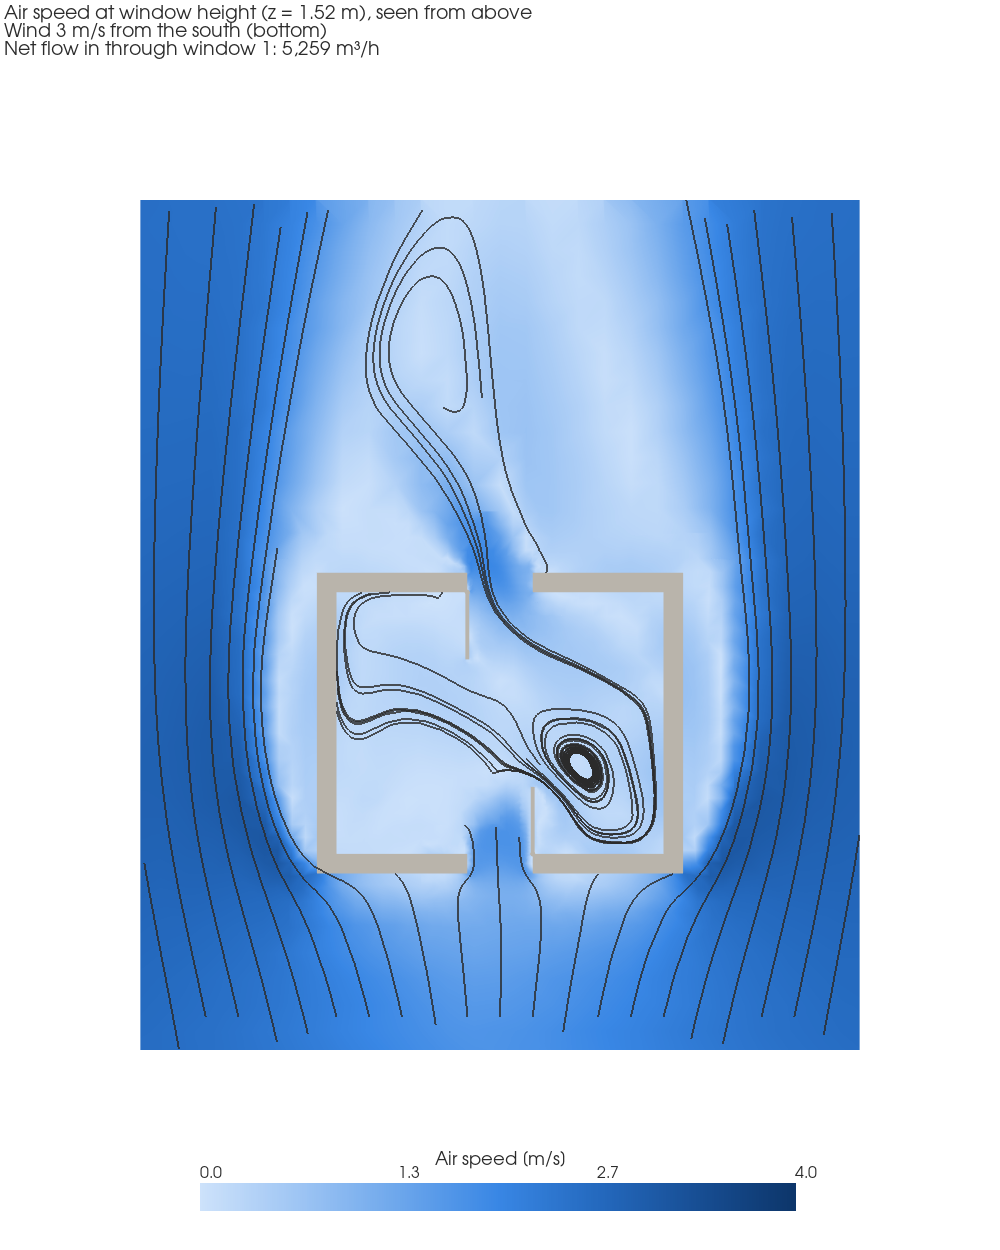
\includegraphics[width=\linewidth, trim=138 198 138 198, clip]{default_flow.png}
\captionof{figure}{\raggedright Example case seen from above at window height. The wind (3\,m/s, from below) enters through one window, crosses the room as a jet and leaves through the opposite window. Colour: air speed from 0 (light) to 4\,m/s (dark); lines: flow paths.}
\end{minipage}

\medskip
% the small labels above the three rooms are cropped away; the caption names the layouts
\begin{center}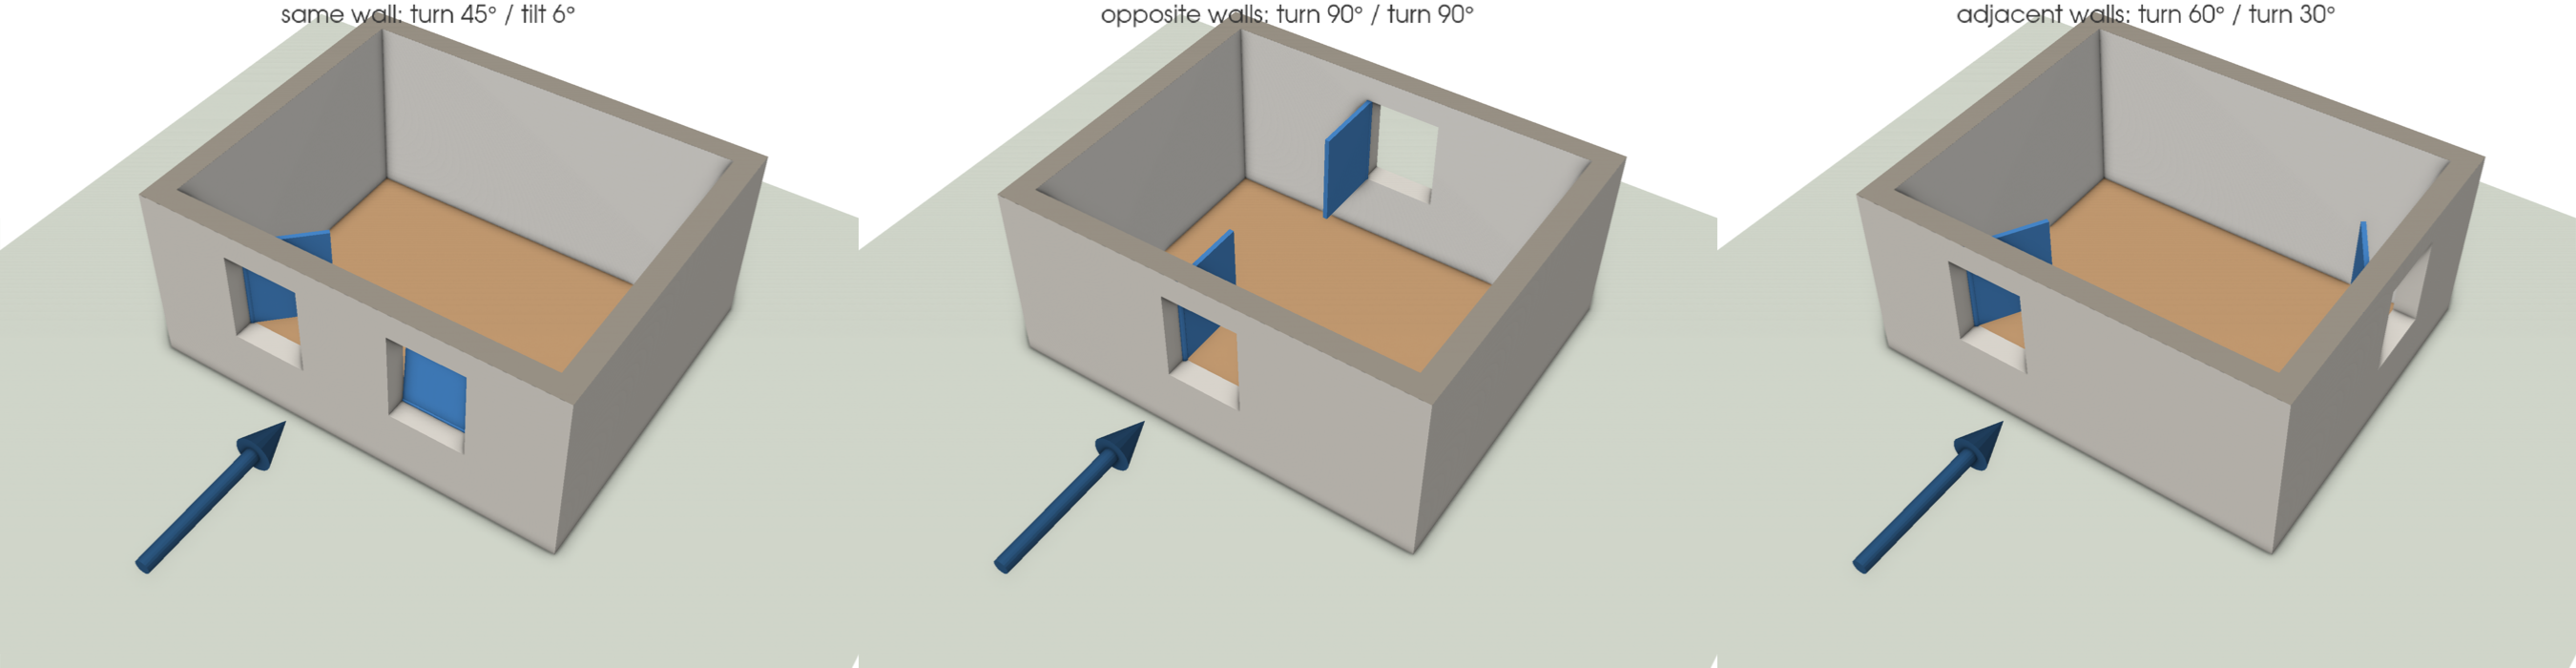
\includegraphics[width=0.86\textwidth, trim=0 0 0 75, clip]{layouts.png}\end{center}\vspace{-14pt}
\captionof{figure}{The simulated room (5\,×\,4\,×\,2.5\,m, roof removed) with windows on the same wall, on opposite walls and on adjacent walls. Blue plates: opened windows. Arrow: wind.}

\head{Process: one simulation, fully automatic}
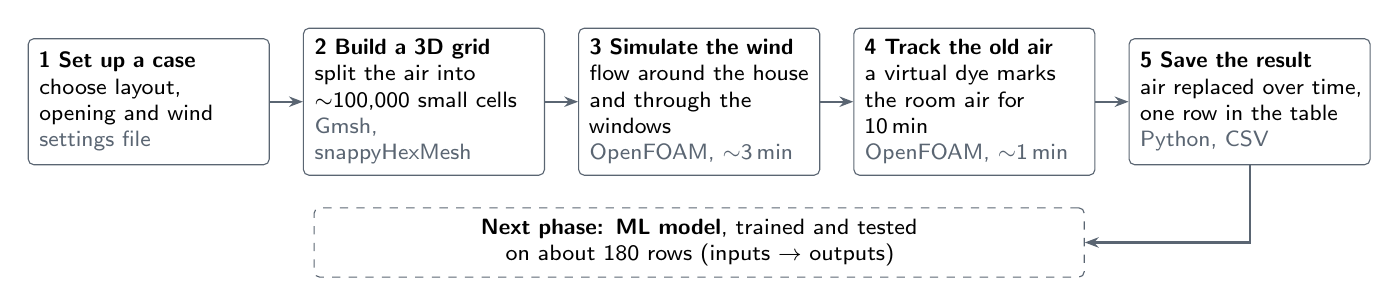
\begin{tikzpicture}[
    box/.style={draw=muted, rounded corners=2pt, text width=2.78cm, minimum height=1.6cm,
                align=left, inner sep=4pt, font=\footnotesize,
                execute at begin node={\hyphenpenalty=10000}},
    arrow/.style={-{Stealth[length=5pt]}, thick, color=muted},
    node distance=0.42cm]
  \node[box] (s1) {\textbf{1 Set up a case}\\ choose layout, opening and wind\\ {\color{muted}settings file}};
  \node[box, right=of s1] (s2) {\textbf{2 Build a 3D grid}\\ split the air into ${\sim}$100{,}000 small cells\\ {\color{muted}Gmsh, snappyHexMesh}};
  \node[box, right=of s2] (s3) {\textbf{3 Simulate the wind}\\ flow around the house and through the windows\\ {\color{muted}OpenFOAM, ${\sim}$3\,min}};
  \node[box, right=of s3] (s4) {\textbf{4 Track the old air}\\ a virtual dye marks the room air for 10\,min\\ {\color{muted}OpenFOAM, ${\sim}$1\,min}};
  \node[box, right=of s4] (s5) {\textbf{5 Save the result}\\ air replaced over time, one row in the table\\ {\color{muted}Python, CSV}};
  \foreach \a/\b in {s1/s2, s2/s3, s3/s4, s4/s5} \draw[arrow] (\a) -- (\b);
  \node[draw=muted, dashed, rounded corners=2pt, below=0.4cm of s3, text width=9.5cm, align=center,
        inner sep=4pt, font=\footnotesize] (ml)
        {\textbf{Next phase: ML model}, trained and tested on about 180 rows (inputs $\to$ outputs)};
  \draw[arrow] (s5.south) |- (ml.east);
\end{tikzpicture}

\head{Checks before the big run}
A simulation can give wrong numbers that still look reasonable, so we tested how far the results can be trusted.

\renewcommand{\arraystretch}{1.2}
\begin{tabularx}{\textwidth}{@{}>{\bfseries\raggedright\arraybackslash}p{3.4cm}>{\raggedright\arraybackslash}X@{}}
\toprule
Grid size & Finer or coarser cells change the results by less than 2.5\,\% (our first grid type: 10--20\,\%, so we replaced it). Cases with both windows on the same wall: up to 17\,\%, an extra check is planned. \\
Small changes & Moving a window by 1\,cm changes the result by less than 2.5\,\%. \\
Fast vs.\ exact method\newline\mdseries 12 cases & Averaged wind (${\sim}$5\,min per case) vs.\ wind that changes over time (${\sim}$40\,min): within 3\,\% for windows on different walls, but up to 31\,\% off for windows on the same wall, so those cases will use the exact method. \\
Wind speed & Results scale exactly: three times the wind replaces the air three times as fast (within 3\,\%). \\
Plausibility & Results match textbook formulas for window ventilation and an ideal, perfectly mixed room. \\
\bottomrule
\end{tabularx}

\head{Where we are}
\textbf{Done:} the pipeline runs automatically from a settings file to a table row, and the checks above are complete.\\
\textbf{Next:} final choice of method, then about 180 simulations (about 2 days of computing on one laptop).\\
\textbf{Then:} train and test the ML model on the resulting table.

\end{document}
